\documentclass[12pt]{article}
\usepackage[margin=3cm]{geometry}
\usepackage{graphicx}
\usepackage{float}
\usepackage{url}
\usepackage{listings}
\usepackage{color}

\definecolor{mygreen}{rgb}{0,0.6,0}
\definecolor{mygray}{rgb}{0.5,0.5,0.5}
\definecolor{mymauve}{rgb}{0.58,0,0.82}
\lstset{ %
	xleftmargin=10em,
	backgroundcolor=\color{white},   % choose the background color; you must add \usepackage{color} or \usepackage{xcolor}
	basicstyle=\small,%\footnotesize,        % the size of the fonts that are used for the code
	breakatwhitespace=false,         % sets if automatic breaks should only happen at whitespace
	breaklines=false,                 % sets automatic line breaking
	captionpos=b,                    % sets the caption-position to bottom
	commentstyle=\color{mygreen},    % comment style
	deletekeywords={...},            % if you want to delete keywords from the given language
	escapeinside={\%*}{*)},          % if you want to add LaTeX within your code
	extendedchars=true,              % lets you use non-ASCII characters; for 8-bits encodings only, does not work with UTF-8
	%	frame=single,                    % adds a frame around the code
	keepspaces=true,                 % keeps spaces in text, useful for keeping indentation of code (possibly needs columns=flexible)
	keywordstyle=\color{blue},       % keyword style
	language=C, % the language of the code
	morekeywords={*,...},            % if you want to add more keywords to the set
	numbers=left,                    % where to put the line-numbers; possible values are (none, left, right)
	numbersep=5pt,                   % how far the line-numbers are from the code
	numberstyle=\small\color{mygray}, % the style that is used for the line-numbers
	rulecolor=\color{black},         % if not set, the frame-color may be changed on line-breaks within not-black text (e.g. comments (green here))
	showspaces=false,                % show spaces everywhere adding particular underscores; it overrides 'showstringspaces'
	showstringspaces=false,          % underline spaces within strings only
	showtabs=false,                  % show tabs within strings adding particular underscores
	stepnumber=1,                    % step between two line-numbers. If it's 1, each line will be numbered
	stringstyle=\color{mymauve},     % string literal style
	tabsize=2                  % sets default tabsize to 2 spac                  % show the filename of files included with \lstinputlisting; also try caption instead of title
}

\begin{document}

\begin{titlepage}
	\begin{center}
		
		
		% Upper part of the page. The '~' is needed because \\
		% only works if a paragraph has started.
		\vfill
		
		\textsc{\LARGE Lab 8: Carry-Ripple Addition III}\\[1.5cm]
		
		\Large Adam Sumner\\[0.5cm]
		
		\Large Illinois Institute of Technology\\[0.5cm]
		
		\Large ECE 429-01\\[0.5cm]	
		
		\noindent
		\vfill
		\large \textbf{Lab Date:} November 2\textsuperscript{nd}, 2015\hfill
		\large \textbf{Due Date:} November 11\textsuperscript{th}, 2015
		% Bottom of the page
	
		
	\end{center}
\end{titlepage}

\section{Introduction}
The purpose of this lab is to finalize the design of an adder circuit by combining both the previously designed layout and schematic of a one bit adder from previous labs. Specifically, this lab will tackle building a 4-bit adder circuit. This circuit will then be checked for its accurate functionality using LVS and verilog. 
\section{Theory/Pre-Lab}
\subsection{Theory}
An adder circuit is one that is able to take two binary inputs and accurately calculate the sum. To implement this via circuitry, addition is done bit by bit. As discussed in the previous two experiments a mirror adder circuit design is an efficient way to perform one bit addition with carry. By combining 4 one bit adders, it's possible to add 4 bit numbers together. This is shown in Figure \ref{fig:diagram}.

\begin{figure}[H]
\centering
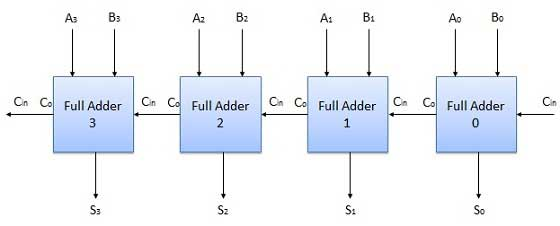
\includegraphics[width=0.7\linewidth]{diagram}
\caption{Four Bit Adder Diagram}
\label{fig:diagram}
\end{figure}

\subsection{Pre-Lab}
The pre-lab involved reviewing the carry-ripple architecture discussed in Lab 6. The following two sets of inputs were also translated:
\begin{itemize}
	\item 11+5
	\item 4+10
\end{itemize} 

\noindent Their translation is shown in Figure \ref{fig:prelab}.

\begin{figure}[H]
\centering
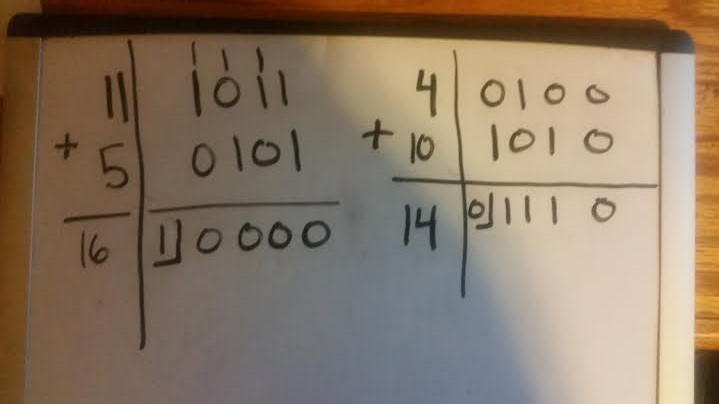
\includegraphics[width=0.7\linewidth]{prelab}
\caption{Pre-Lab Translation}
\label{fig:prelab}
\end{figure}


\section{Implementation}
\subsection{Schematics}
\begin{figure}[H]
\centering
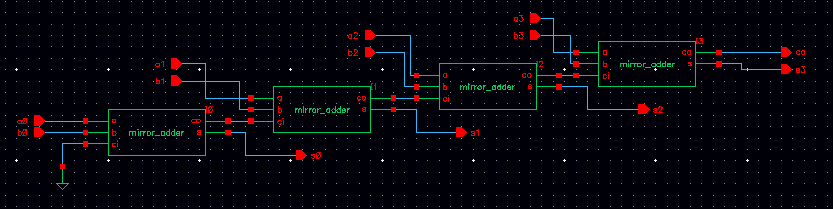
\includegraphics[width=\linewidth]{schematic}
\caption{4-bit Adder Schematic}
\label{fig:schematic}
\end{figure}

\begin{figure}[H]
\centering
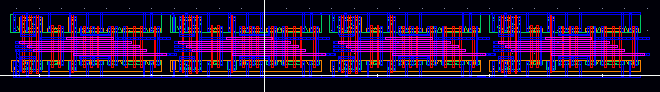
\includegraphics[width=1\linewidth]{layout}
\caption{4-bit Adder Layout}
\label{fig:layout}
\end{figure}

\begin{figure}[H]
\centering
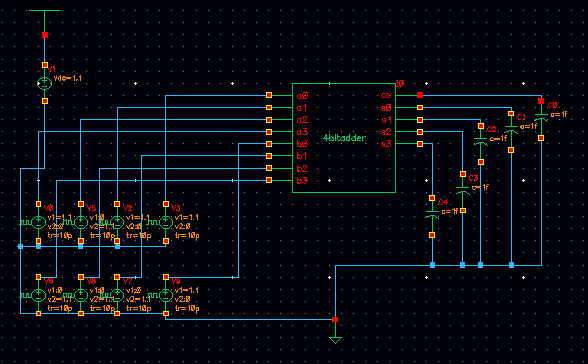
\includegraphics[width=1\linewidth]{test_circuit}
\caption{4-bit Adder Test Circuit ($11+5 \to 4+10$)}
\label{fig:test_circuit}
\end{figure}

\begin{figure}[H]
	\begin{lstlisting}
	module adder_4bit(A,B,S,CO);
		input [3:0] A,B;
		output [3:0] S;
		output CO;
		assign {CO,S}={1'b0,A}+{1'b0,B};
	endmodule
\end{lstlisting}
\caption{Verilog Code for 4-bit Adder Verification}
\label{fig:verilog}
\end{figure}

\begin{figure}[H]
	\begin{lstlisting}
		module stimulus;
			reg [3:0] A,B;
			wire [3:0] S;
			wire CO;
		
			adder_4bit a(A,B,S,CO);
		
			initial
			begin
				#10 A=4'b0000; B=4'b0000;
				#5 $display("%d+%d=%d %b", A,B,S,CO);
		
				#10 A=4'b1011; B=4'b0101;
				#5 $display("%d+%d=%d %b", A,B,S,CO);
		
				#10 A=4'b0100; B=4'b1010;
				#5 $display("%d+%d=%d %b", A,B,S,CO);
		
				#10 A=4'b0001; B=4'b0001;
				#5 $display("%d+%d=%d %b", A,B,S,CO);
		
				#10 A=4'b0001; B=4'b0111;
				#5 $display("%d+%d=%d %b", A,B,S,CO);
		
				#10 A=4'b1000; B=4'b0111;
				#5 $display("%d+%d=%d %b", A,B,S,CO);
			end
		endmodule
	\end{lstlisting}
	\caption{Verilog Code for 4-bit Adder Verification}
	\label{fig:verilog_stim}
\end{figure}


\subsection{Procedure}
The procedure of this lab involved first constructing the schematic and layout of the 4-bit adder. This is shown in Figures \ref{fig:schematic} and \ref{fig:layout}. LVS was then run to verify that they are both equivalent. After this, two verilog files shown in Figures \ref{fig:verilog} and \ref{fig:verilog_stim} were created and verified using the command: \\ ~\\ \texttt{verilog adder4\textbackslash\  test.v adder4.v} \\ ~\\
Once this was done, ESP was run to check that the schematic functionality was the same of the verilog functionality. Once done, a test circuit was created to simulate 11+4 and 4+10. This is shown in Figure \ref{fig:test_circuit}. Once all the functionality of the adder was verified, the delay was calculated between the CO signal and S signals with the input A signals.
\subsection{Results}
\begin{figure}[H]
\centering
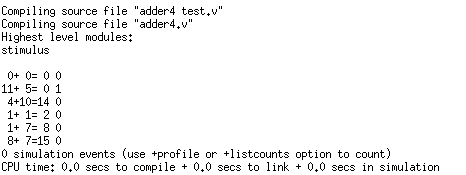
\includegraphics[width=1\linewidth]{verilog_verification}
\caption{Verilog Verification}
\label{fig:verilog_verification}
\end{figure}

\begin{figure}[H]
\centering
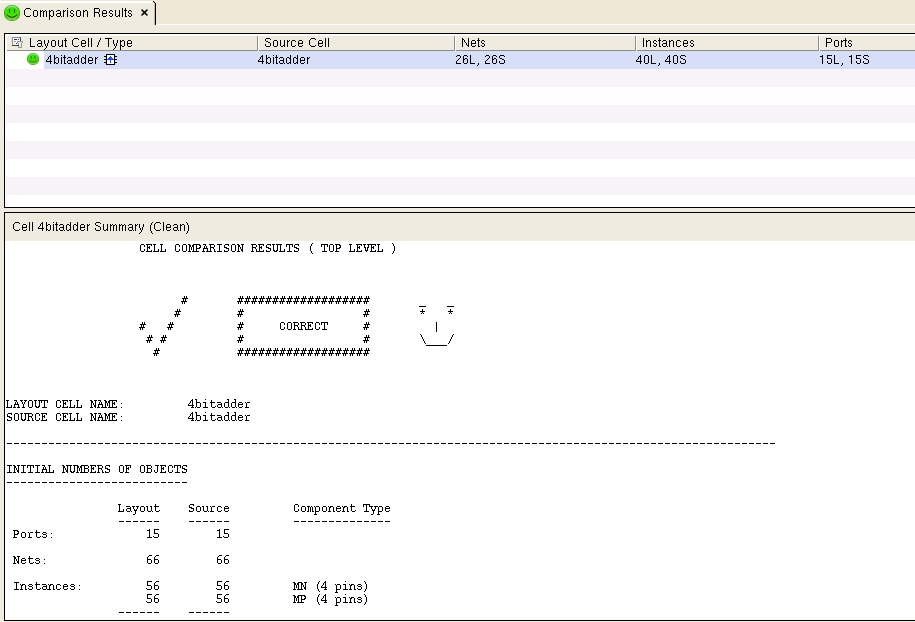
\includegraphics[width=1\linewidth]{LVS}
\caption{LVS Verification}
\label{fig:LVS}
\end{figure}

\begin{figure}[H]
\centering
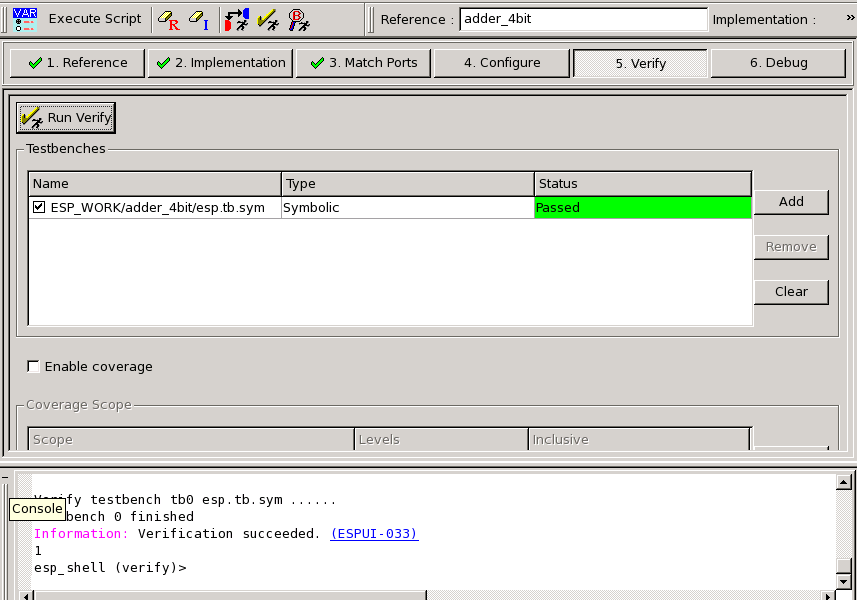
\includegraphics[width=1\linewidth]{esp}
\caption{Equivalence Checking using ESP}
\label{fig:esp}
\end{figure}



\subsection{Discussion}

%\subsection{Bonus Work}
\section{Conclusions}


\end{document}
